\section{Protocol Security}
\label{sec:security}

Yao's protocol is designed to provide \ac{SFE} against \emph{semi-honest} adversaries. These security guarantees do not carry over against \emph{malicious} adversaries.  This is a serious limitation for making the protocol practical; there are relatively few real-world scenarios where you \emph{do not} trust the other party to see your inputs to a function, but \emph{do} trust them to forgo the opportunity to discover those same inputs by deviating from the protocol.

Much work has been conducted to extend Yao's protocol to be secure against \emph{malicious} adversaries.  This work can generally be classified into three areas, 1) creating \emph{1-out-of-2 \ac{OT}} protocols that are secure against \emph{malicious} adversaries, 2) ensuring that the circuit constructing party correctly constructs the garbled circuit, and 3) preventing \ac{P1} from gaining an advantage by sending \ac{P2} corrupt values for her input.

Finally, some discussion is given to the open problem of how to guarantee \emph{fairness} in the \emph{malicious} case, by ensuring \ac{P2} returns output to \ac{P1} at the end of the protocol.

\subsection{Securing the \ac{OT} Protocol}
\label{sec:securingot}

The \emph{1-out-of-2 \ac{OT}} protocol described in the section \ref{sec:ot} is trivially vulnerable in the \emph{malicious} case.  Instead of generating $((k^{pub}_b, k^{pri}_b), (k^\bot_{b-1}, \bot))$, \ac{P2} could easily generate two valid public / private key pairs, allowing her to recover both values sent by \ac{P1}. Applied to Yao's protocol, this would allow \ac{P2} to learn both the garbled versions of the 0 and 1 values for all of her input bits. \ac{P2} having these additional keys would allow \ac{P2} to decrypt additional values throughout the circuit, violating the \emph{privacy} requirement of \ac{SFE}.  Others have detailed several additional ways that using an insecure-in-the-\emph{malicious}-case \ac{OT} protocol can be exploited by an attacker\cite{kiraz2006protocol}.

As previously discussed, \ac{OT} is a distinct, though related, field to both \ac{SFE} and Yao's protocol.  As such, this section does not attempt to assess the state-of-the-art in \ac{OT}.  A variety of other approaches to \emph{malicious}-case secure \emph{1-out-of-2 \ac{OT}} protocols exist\cite{naor2001efficient, kiraz2006protocol, goldreich1987play, naor2005computationally}, each with their own requirements, computation costs and underlying security assumptions.  The below protocol\cite{bellare1990non}\footnote{This protocol is a slightly modified version of the protocol presented in \cite{bellare1990non}.  It incorporates a change suggested by \cite{naor2001efficient} to remove the reliance on a external zero knowledge proof or other out-side-the-protocol source for \emph{C}.} is included to show that efficient \emph{1-out-of-2 \ac{OT}} with \emph{malicious} adversaries is possible, and that researchers have used it and equivalent \ac{OT} protocols to make Yao's protocol secure in the \emph{malicious} case.

\begin{algorithm}[H]
    \floatname{algorithm}{Protocol}
    \caption{Malicious-Secure 1-out-of-2 Oblivious Transfer}
    \label{alg:otmalicious}
    \begin{algorithmic}[1]
        \STATE \ac{P1} has a set of two strings, $S = \{s_0, s_1\}$.
        \STATE \ac{P1} (sender) and \ac{P2} (receiver) agree on some $q$ and $g$ such that $g$ is a generator for $\mathbb{Z}^*_q$.
        \STATE \ac{P1} selects a value  $C$ from $\mathbb{Z}^*_q$ such that \ac{P2} does not know the discrete log of $C$ in $\mathbb{Z}^*_q$.
        \STATE \ac{P2} selects $i \in \{0, 1\}$ corresponding to whether \ac{P2} wants $s_0$ or $s_1$. \ac{P2} also selects a random $0 \leq x_i \leq q-2$.
        \STATE \ac{P2} sets $\beta_i = g^{x_i}$ and $\beta_{i-1} = C \odot (g^{x_i})^{-1}$. $(\beta_0, \beta_1)$ and $(i, x_i)$ form \ac{P1} public and private keys, respectively.

        \STATE \ac{P1} checks the validity of \ac{P2}'s public keys by verifying that $\beta_0 \bullet \beta_1 = C$.  If not, \ac{P1} aborts.

        \STATE \ac{P1} selects $y_0, y_1$ such that $0 \leq y_0, y_1 \leq q-2$, and sends \ac{P2} $a_0 = g^{y_0}$ and $a_1 = g^{y_1}$.
        \STATE \ac{P1} also generates $z_0 = \beta^{y_0}_0, z_1 = \beta^{y_1}_1$ and sends \ac{P2} $r_0 = s_0 \oplus z_0$ and $r_1 = s_1 \oplus z_1$.
        \STATE \ac{P2} computes $z_i = a^{xi}_i$ and then receives $s_i$ by computing $s_i = z_i \oplus r_i$.
    \end{algorithmic}
\end{algorithm}

The purpose of many of the steps in the protocol are not explicit in the original work\cite{bellare1990non}, so some explanation is provided below.  Specifically, in step 5 \ac{P1} checks that $\beta_0 \bullet \beta_1 = C$ to prevent \ac{P2} from being able to decrypt under both $\beta_0$ and $\beta_1$, and to force \ac{P2} to choose one or the other. As long as the assumption that \ac{P2} does not know the discrete log of $C$ holds, then it follows that \ac{P2} cannot know the discrete log of both $\beta_0$ and $\beta_1$.

Steps 7, 8 and 9 function similarly to a Diffie-Hellman key exchange.  However, in step 9 it may not be immediately obvious why \ac{P2} is able to reconstruct $z_i$ to decrypt $r_i$ and receive $s_i$.  To understand why, recall that $a_i$ is equal to $g^{y_i}$, making $a^{y_i}_i = g^{y^{x_i}_i} = g^{y_i \bullet x_i}$.

Similarly , recall that $z_i$ was generated from $B^{y_i}_i$ and that $B_i = g^{x_i}$.  This makes $B^{y_i}_i = g^{x^{y_i}_i} = g^{x_i \bullet y_i}$.  Since \ac{P2} is able to construct the same pad \ac{P1} used to mask $s_i$, \ac{P2} can undo the mask and receive $s_i$.


\subsection{Securing Circuit Construction}
\label{sec:securingcircuits}

A second way a malicious adversary could exploit Yao's protocol to learn information about the other party's input is by \ac{P1} creating and garbling a circuit for a function other than the function expected by \ac{P2}. Trivially, \ac{P1} could send \ac{P2} a garbled circuit that echos back \ac{P2}'s input.  More reasonably, \ac{P1} could construct the circuit to output a value that leaks information about $i_{P2}$ in some less obvious manner not known to \ac{P2}.  It is therefor necessary for \ac{P2} to ensure that the garbled circuit she evaluates is actually modeling the expected function.

\subsubsection{Zero-Knowledge Proofs}

Two different general strategies for achieving this assurance have been promoted.  The first approach has \ac{P1} generate a zero knowledge proof of the garbled circuit's correctness, and then sends this proof to \ac{P2} along with the garbled circuit and \ac{P1}'s garbled inputs\cite{goldreich1987play, goldreich2009foundations}.

This zero-knowledge strategy dates back to earlier in the history of Yao's protocol, when the protocol served more as proof that \ac{SFE} was possible and less as a practical tool for actually achieving \ac{SFE}. More recent, implementation-focused work on Yao's protocol has treated the zero-knowledge proof approaches as too expensive for practical use\cite{lindell2007efficient, mohassel2006efficiency, malkhi2004fairplay}, and thus this strategy is not discussed further in this paper.

\subsubsection{Cut-and-Choose}
\label{sec:cutchoosesimple}

Instead, recent work on Yao's protocol has focused on a \emph{cut-and-choose} strategy for securing circuit construction\cite{malkhi2004fairplay}. Work on this approach has developed in an arms-race fashion, with proposals being made, other researchers revealing shortcomings in the given strategy, and a revised strategy being developed to address the given weakness. Several rounds of this propose-attack-revise cycle are discussed below, to better explain the role of each proposed improvement.\\[.5em]

\noindent\textbf{Standard Cut-and-Choose}

Under this approach, \ac{P1} constructs $m$ versions of the circuit, each structured identically but garbled differently so that the keys for each gate in each circuit are unique. \ac{P1} does the same for his inputs to each of the $m$ garbled circuits. Additionally, \ac{P1} generates a ``commitment'' for each of his garbled inputs, which for simplicity can be understood to be a simple hash of the inputs\footnote{Though several more secure methods of committing are mentioned in \cite{lindell2007efficient}, a simple hash function is used here to simplify the description of the cut-and-choose approach here, and commitment schemes in general throughout this paper.  A more secure approach is described in \cite{halevi1996practical}.}.

\ac{P1} then sends each of these pairs of garbled circuits and associated input commitments to \ac{P2}, who selects $m-1$ versions of the circuit to verify.  \ac{P1} de-garbles each of the $m-1$ selected circuits, so that \ac{P2} can see the underlying circuit with the now unobscured boolean values in each gates' computation table.  \ac{P2} can then verify that each of the revealed circuits are constructed correctly and as expected.

If everything looks correct to \ac{P2} she will continue with the computation by receiving \ac{P1}'s garbled inputs, checking that they match their corresponding, previously sent commitment (again, most simply thought of as checking that the hash of the received garbled inputs matches the previously sent hash), and then proceed with Yao's protocol as normal. This reduces the chances of \ac{P1} tricking \ac{P2} into computing a corrupted circuit to $1/m$. This protocol is described more formally in protocol \ref{alg:cutandchoose-basic}.

\begin{algorithm}[H]
    \floatname{algorithm}{Protocol}
    \caption{Securing Circuit Construction With Cut-and-Choose}
    \label{alg:cutandchoose-basic}
    \begin{algorithmic}[1]
        \STATE \ac{P1} generates $m$ garbled versions of the circuit $c$, along with a corresponding garbled version of his input, called $X_i$ for $0 \leq i < m$.
        \STATE \ac{P1} uses hash function $H$ to generate commitments to each garbled input, $COM_i = H(X_i)$ for $0 \leq i < m$.

        \STATE \ac{P1} sends \ac{P2} $m$ garbled circuits and $COM$ such that $|COM| = m$.
        \STATE \ac{P2} selects $0 \leq j < m$ and \ac{P1} un-garbles all circuits except the $j$th.
        \STATE \ac{P2} inspects all $m-1$ circuits to check that they are correctly formed. If not, \ac{P2} aborts.

        \STATE \ac{P2} receives \ac{P1}'s garbled inputs to circuit $j$ and confirms that \ac{P1} did not change his inputs by verifying $COM_j = H(X_j)$. If not, \ac{P2} aborts.

        \STATE Otherwise, \ac{P2} receives the continues with Yao's protocol as normal.
    \end{algorithmic}
\end{algorithm}


\noindent\textbf{Further Securing Cut-and-Choose}

However, for many applications one may wish for a stronger guarantee against executing a malicious circuit from \ac{P1}.  Lindell and Pinkas\cite{lindell2007efficient} discovered that \ac{P1}'s odds of success can be dramatically reduced without the overhead of needing to generate additional circuits by altering the cut-and-choose strategy slightly.

Instead of \ac{P1} revealing $m-1$ circuits, Lindell and Pinkas have \ac{P2} select only $m/2$ circuits to be revealed.  \ac{P2} computes the remaining $m/2$ circuits and takes the majority result. Under this construction, a malicious \ac{P1} would only succeed in having \ac{P2} output a corrupt result if

\begin{enumerate*}
    \item \ac{P1} constructs more than $m/4$ of the circuits corruptly, and
    \item None of the corrupt $m/4$ circuits are among the $m/2$ circuits \ac{P2} selected to be revealed.
\end{enumerate*}

Lindell and Pinkas measure \ac{P1}'s chance of success in such an attack at $2^{-0.311m}$, where $m$ is the number of circuits generated\cite{lindell2007efficient}.\\[.5em]

\noindent\textbf{Majority Result as a Defense Against a Malicious Circuit}

An immediate question that comes out of the above approach is why \ac{P2} should take the majority result of the computed $m/2$ circuits, instead of immediately aborting when encountering the first corrupt circuit, especially given that computing a garbled circuit is an expensive operation.  The reason is that, were \ac{P2} to abort if all circuit outputs were not identical, she would become vulnerable to a different attack from \ac{P1}.

Consider the case where \ac{P1} constructs all circuits correctly, with a single exception.  This corrupt circuit outputs the correct value of the function $\oplus$'ed with the first bit of \ac{P2}'s input.  By observing whether \ac{P2} evaluates all $m/2$ evaluation-circuits, \ac{P1} learns the first bit of \ac{P2}'s input.

\begin{figure}[t]
    \centering
    \begin{tabular}{ c | c | c || c | l }
        \hline
        $f_0$ & $i_{P2_0}$ & $f_0 \oplus i_{P2_0}$ & \ac{P2} returns & \ac{P1} learns \\
        \hline
        0 & 0 & 0 & 0 & $i_{P2_0} = 0$\\
        \hline
        0 & 1 & 1 & $\bot$ & $i_{P2_0} = 1$\\
        \hline
        1 & 0 & 1 & 1 & $i_{P2_0} = 0$\\
        \hline
        1 & 1 & 0 & $\bot$ & $i_{P2_0} = 1$\\
        \hline
    \end{tabular}
    \caption{Using a corrupted circuit to learn first bit of \ac{P2}'s input}
    \label{fig:earlyabortattack}
\end{figure}

Figure \ref{fig:earlyabortattack} provides a full explanation of how \ac{P1} performs this attack.  The first column depicts the first bit of the correct value returned by $f$, and the second column shows the first bit of \ac{P2}'s input.  The third column shows the first bit of the value returned by \ac{P1}'s malicious circuit, and column four describes the value \ac{P2} returns from evaluating the entire $m/2$ set of circuits (or $\bot$ if \ac{P2} aborts).  Finally, column five shows what \ac{P1} is able to learn about \ac{P2}'s input, without having access to the first three columns of the table.\\[.5em]


\noindent\textbf{Further Work Ensuring Consistent Inputs From \ac{P1}}

Lindell and Pinkas's\cite{lindell2007efficient} solution of having \ac{P1} provide $m$ versions of the garbled circuit succeeds in providing \ac{P2} with a high degree of confidence that \ac{P1} has not corrupted any circuits.  However, it leads to another problem, of ensuring that \ac{P1} provides the same input to each of the circuits \ac{P2} evaluates.  Solutions to this problem involve additional, involved protocols\cite{lindell2007efficient} or rely on other areas of cryptography\cite{shen2011two} that are beyond the scope of this paper.  More discussion of this problem, as well as possible solutions to it, are provided by other work\cite{kreuter2012billion}.


\subsection{Securing Against Corrupt Inputs}
\label{sub:inputattacks}

A third area where a malicious party can exploit the original construction of Yao's protocol is in the values \ac{P1} returns to \ac{P2} in the \emph{1-out-of-2 \ac{OT}} step.  Recall that this \ac{OT} step is taken to prevent \ac{P1} from learning whether \ac{P2} is requesting the garbled value for a 0 or a 1 bit in her input.  The protections given in the previous two subsections provide no security against this attack. Subsection \ref{sec:securingot} only addresses ensuring that \ac{P1} cannot learn \ac{P2}'s inputs \emph{during} the \ac{OT} step, not that these inputs cannot be leaked elsewhere in the protocol.  Subsection \ref{sec:securingcircuits} provides \ac{P2} guarantees that the circuits being evaluated are not corrupt, but provides no guarantees that the inputs to those circuits are not corrupt.

\ac{P1} can exploit this weakness in the protocol to gain information about \ac{P2}'s input in the following manner.  Instead of returning \ac{P2} the correct garbled values for each bit of her input, \ac{P1} returns the correct garbled value for 0, and a corrupt value for 1.  \ac{P1} can then learn whether \ac{P2} received the 0 or 1 value by observing if \ac{P2} aborts while computing the circuit.  If \ac{P2} received the 0 value, she will be able to compute the circuit as normal; if \ac{P2} received the 1 value, she will not be able to compute the circuit and will be forced to abort.  Either way, \ac{P1} is able to learn the value of a bit of \ac{P2}'s input.

\begin{figure}
    \centering
    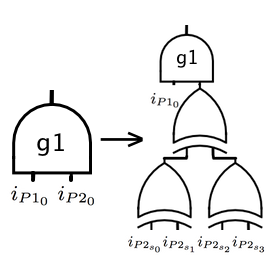
\includegraphics[width=\columnwidth]{images/secureing_malicious_inputs}
    \caption{Securing against \ac{P1} providing malicious inputs through $s$ new $\oplus$ gates}
    \label{fig:inputsecure}
\end{figure}

Lindell and Pinkas\cite{lindell2007efficient} provide a method of securing the protocol against this attack.  Their technique is depicted in figure \ref{fig:inputsecure}.  The defense works by adding $s|i_{P2}|$ input bits to the circuit, where $s$ is a chosen security parameter.  Each of \ac{P2}'s input bits is replaced by the result of XOR of $s$ new input bits, each chosen by \ac{P2} from \ac{P1} through the same \ac{OT} protocol.  The circuit is also augmented to reflect these new input wires and XOR gates. This step of indirection gives \ac{P2} $2^{s-1}$ ways to receive her true input bits from \ac{P1}, and prevents \ac{P1} from gaining any knowledge about \ac{P2}'s underlying input bit by corrupting the augmented, XORed inputs.

Note that this construction does not prevent \ac{P1} from forcing \ac{P2} to abort when executing the circuit, it only prevents \ac{P1} from learning anything about \ac{P2}'s input.


\subsection{Ensuring \ac{P2} Returns At All}

One remaining problem with Yao's protocol in the \emph{malicious} setting is how to ensure \ac{P2} returns to \ac{P1} any output value from the function.  There is no clear method to prevent \ac{P2} from maliciously aborting the protocol early, right after computing the output of the garbled circuit, but right before sending the output to \ac{P1}.  That this problem is still open means that the \emph{fairness} principle Yao described for \ac{SFE} cannot be guaranteed in the \emph{malicious} setting.

As a second best option, much work has been done to ensure that if \ac{P2} does output a value, it is the correct computation returned by the function\cite{shen2011two}.  Another possibility though is that, until a solution to this problem is found, Yao's protocol is only appropriate in the \emph{malicious} setting where the inputs to the function need to be kept private, but the output does not.  An example of such a scenario is a secure voting systems.  However, this restriction clearly limits the number of problems for which Yao's protocol is appropriate.

